% This text is proprietary.
% It's a part of presentation made by myself.
% It may not used commercial.
% The noncommercial use such as private and study is free
% Sep. 2005 
% Author: Sascha Frank 
% University Freiburg 
% www.informatik.uni-freiburg.de/~frank/
% additional use of \usepackage{beamerthemesplit}
\documentclass{beamer}
\usepackage[utf8]{inputenc}
\usepackage[T2A]{fontenc} % кодировка шрифта
\usepackage[english,russian]{babel} % язык документа
\usepackage{beamerthemesplit}
\usepackage{graphicx}
\usefonttheme{professionalfonts}

\theoremstyle{plain}
\newtheorem{thm}{Теорема}[section]

\usepackage{beamerthemesplit} % new 
\begin{document}

\title{Задача о многоруком бандите} 
\author{Васильев Павел, Стахеев Константин}


 
\date{14 мая 2024 г.} 

\frame{\titlepage}

\section{Постановка задачи}
\frame{ 
Есть $n$ игровых автоматов. Дёргая ручку $i = 1, ..., n$ мы каждый раз с вероятностью $p_i$ получаем 1 рубль, а с вероятностью $1-p_i$ не получаем ничего. Разрешается сделать $N >> 1$ шагов, на каждом шаге можно дёргать только одну ручку. Сами $p_i$ априорно не известны. Но мы знаем, что $p_i \sim U[0,1]$. Нужно найти стратегию выбора ручек такую, чтобы максимизировать доход.

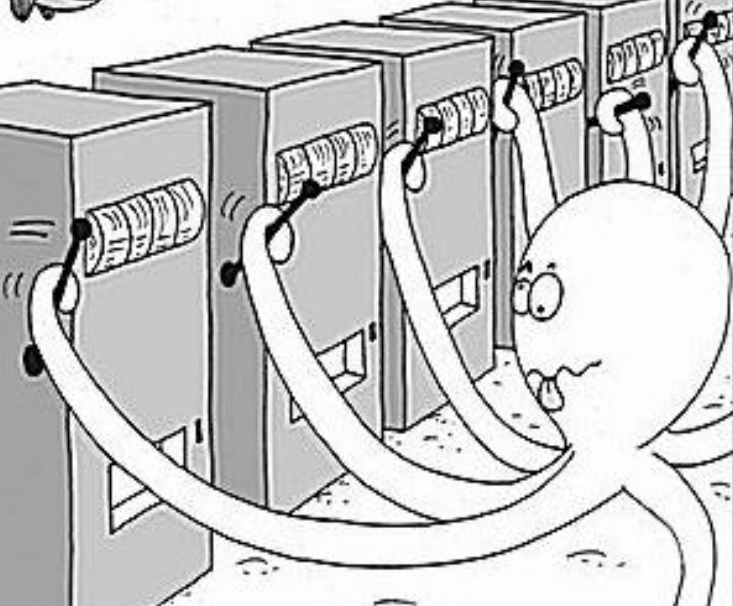
\includegraphics[width=5cm]{multi_armed_bandit.png}

}

\frame{

Первая идея - давайте изучим все ручки, а затем жадно будем выбирать ту, которая в среднем даёт лучшую награду, и будем всегда её выбирать

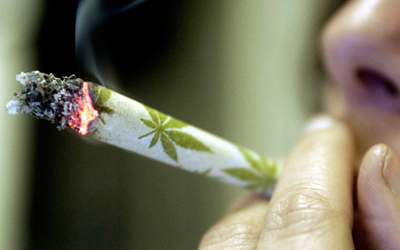
\includegraphics[width=4cm]{kosjak.jpg}
}


\frame{

Проблема: как понимать, сколько раз мы будем изучать эти действия до того, как начнем пользоваться.
}

\section*{Слово про управляемые марковские процессы}
\frame{
\frametitle{Слово про управляемые марковские процессы}

$S$ - конечноче множество состояний.

В момент времени $t = 0, 1, ...$ система претерпевает изменения, и на каждом шаге мы вольны выбирать состояние исходя из своей стратегии и истории переходов.

\begin{itemize}
\item $s$ - исходное состояние
\item $a$ - действие, переводящее состояние агента из состояния $s$ в $s'$ в момент времени $t$ 
\end{itemize}

\[ \sum_{s' \in S} p(s,a;s') = 1 \]
}

\frame{
\frametitle{Слово про управляемые марковские процессы}

В каждый момент времени мы получаем вознаграждение $r(s,a)$

Цель - получить максимальное итоговое вознаграждение:

\[ V^*(s) = \max_{a} \mathbb{E} \sum_{t=0}^\infty \gamma^t r(s_t, a(s_t)), \quad s_0 = s \]

$\gamma \in (0,1]$ - инфляция
}

\frame{
\begin{equation}
\begin{gathered}
V^*(s_0) = \max_{a} \mathbb{E} \sum_{t=0}^\infty \gamma^t r(s_t, a(s_t)) = \\
= \max_{a} \mathbb{E} \left( r(s_0, a(s_0)) + \gamma \sum_{t=0}^\infty \gamma^t r(s_{t+1}, a(s_{t+1})) \right) =\\
 = \max_{a} (R(s_0, a) + \gamma \mathbb{E}_{s_1} V^*(s_1)) =\\
\max_{a} \left( R(s_0, a) + \gamma \sum_{s_1}p(s,a;s_1)V^*(s_1) \right)
\end{gathered}
\end{equation}
}

\section{Ближе к задачке}
\frame{

Нужно сопоставить описание процесса выбора ручек с управляемым марковским процессом и получить соответствующее уравнение Вальда-Беллмана.

Пространства состояний: $w$-win, $l$-lose.

\[ s = (w_1, l_1; ...; w_n, l_n) \]

\[ \sum_{i=1}^n (w_i + l_i) = k \]

\begin{itemize}
\item $k$ - номер шага
\item $w_i$ - то, сколько выигрышей было связано с $i$-ой ручкой к $k$-ому шагу
\item $l_i$ - сколько неудач принесла $i$-ая ручка к шагу $k$
\end{itemize}
}

\frame{
\frametitle{Ближе к задачке}

Стратегия  - это выбор на каждом шаге одной из ручек $a(s) \in \{ 1, ..., n \}$.

При этом мы ничего не знаем про вероятности переходов из одного состояния в другое:

\[ (w_1, l_1; ..., w_i, l_i; ...; w_n,l_n) \rightarrow (w_1, l_1; ...; w_i+1, l_i; ...; w_n,l_n) \]

\[ (w_1, l_1; ..., w_i, l_i; ...; w_n,l_n) \rightarrow (w_1, l_1; ...; w_i, l_i+1; ...; w_n,l_n) \]

Пусть 

\[ \rho_i^w (w_i, l_i) = P(w_i \leftarrow w_i+1) \]
\[\rho_i^l (w_i, l_i) = P(l_i \leftarrow l_i+1)\]

}

\frame{

В нашей задаче уравнение Вальда-Беллмана будет иметь такой вид:


\includegraphics[width=2cm]{skip.png}

\begin{equation}
\begin{gathered}
V^*(w_1, l_1; ...;w_n, l_n) = \\
= \max_{i=1,...,n} \mathbb{E}_{\rho_i^w, \rho_i^l} ( \rho_i^w(w_i, l_i) \cdot \left( 1+\gamma V^*(w_1, l_1;...;w_i+1,l_i;...;w_n,l_n) \right) +\\
+ \rho_i^l(w_i, l_i) \gamma V^*(w_1,l_1;...;w_i,l_i+1;...;w_n,l_n) | (w_i, l_i) )
\end{gathered}
\end{equation}

Решение такого уравнения дорогое экспоненциально.

}

\subsection{Две ручки}
\frame{
\frametitle{Две ручки}
Рассмотрим случай, когда всего 2 ручки, вероятность на одной из которых известна и равна $p$.

Выигрыш: $V^*(w,l;p)$

Тогда уравнение Вальда-Беллмана будет такое:

\begin{equation}
\begin{gathered}
V^*(w,l;p) = \max ( \frac{p}{1-\gamma},\\ \frac{w+1}{w+l+2} [1+\gamma V^*(w+1,l;p)] + \frac{l+1}{w+l+2}\gamma V^*(w,l+1;p) )
\end{gathered}
\end{equation}

При $w+l>>1$ $V^*(w,l;p)$ недалеко от $(1-\gamma)^{-1} \max \left( p, \frac{w}{w+l} \right)$

}

\frame{
\frametitle{Индекс Гиттинса}

\[ \gamma < 1 \]

\[ V^*(w,l;p) = \frac{p}{1-\gamma} \]

Индекс Гиттинса - это решение этого уравнения.

Есть некая гарантированная сумма выигрыша.
Индекс Гиттинса предлагает очевидную стратегию поведения в казино: всегда играйте на автомате с наивысшим индексом.

Индекс Гиттинса дает нам формальное обоснование, почему мы всегда предпочитаем узнавать нечто новое при условии, что у нас есть некоторая возможность воспользоваться результатами исследования. 
}


\frame{

Введём $Q$-функцию

\[ Q(s,a) = \sum_{s' \in S} p(s,a;s') \left(r(s,a;s') + \gamma V^*(s') \right) \]

\[ V^*(s) =  \max_{a} Q(s,a) \]

}

\frame{
\[Q(s,a) = \sum_{s' \in S} p(s,a;s') \left( r(s,a;s') + \gamma \max_{a'} Q(s', a') \right) \]

Это уравнение можно решить методом последовательных итераций. Можно смотреть на $Q = \{ Q(s,a) \}_{s \in S, a \in A}$ как на вектор. Тогда надо решить уравнение 
\[ Q = H(Q) \]

где $H$ - сжимающий оператор, который мы не можем посчитать явно.

\[ Q_{t+1} = H(Q_t) \]
}

\frame{

Суть $Q$-обучения - заменить невычислимое $H(Q_t)$ (так как мы не знаем $H$) на его вычислимую несмещённую оценку:

\begin{equation}
\begin{gathered}
Q_{t+1}(s,a) = Q_t(s,a) + \\
+ \alpha_t(s,a) \left( r(s,a;s'(s,a)) + \gamma \max_{a'} Q_t(s'(s,a), a') - Q_t(s,a) \right)
\end{gathered}
\end{equation}

\[ \text{НоваяОценка := СтараяОценка + Шаг[Цель-СтараяОценка]} \]


Здесь $s'(s,a)$ - положение процесса на шаге $t+1$, если на шаге $t$ процесс был в состоянии $s$ и было выбрано действие $a$.

Тут всё умеем считать.

}

\frame{

Если $(s, a)$ будет бесконечное число раз встречаться, то хотим

\[ \sum_{t=0}^\infty \alpha_t(s, a) = \infty \]

\[ \sum_{t=0}^\infty \alpha_t^2(s,a) < \infty  \]

Тогда процесс $Q_{t+1} = H(Q_t)$ сойдётся:

\[ \lim_{t \rightarrow \infty} Q_t(s,a) = Q(s,a) \]

}

\frame{

Проделав большое число шагов, мы можем определить оптимальную стратегию, не зная никакую информацию про управляемый марковский процесс.

Правда проблема в том, что мы не знаем, сколько шагов нужно сделать, чтобы считать, что можно закончить обучение. Мы не знаем, в какой момент можно переходить на стратегию 

\[ a_t(s) = \arg \max_{a} Q_t(s,a) \]

}

\subsection{Исходная постановка}
\frame{
\frametitle{Асимптотические оценки}

Будем считать $\gamma = 1$.
Пусть нам дали $N$ шагов и предположим, что мы знаем оптимальную ручку (у неё успех $p_{\max}$). Тогда можем получить ожидаемое вознаграждение $p_{\max} N$. 
Оказывается, что если мы ничего о ручках не знаем, то мы не сможем получить ожидаемое вознаграждение больше, чем

\[ p_{\max} N - 0.05\sqrt{Nn} \]

Как можно приблизиться к такой оценке? 
\begin{itemize}
\item Алгоритм $Exp3$ обеспечивает вознаграждение не меньше чем \[ p_{\max}N - 2\sqrt{Nn \ln n} \]
\end{itemize}
}



\subsection{Стратегии}
\frame{
\frametitle{Ещё стратегии}
\begin{itemize}
\item Сэмплирование по Томпсону
\item $\varepsilon$-жадный алгоритм
\item $Softmax$
\item Доверительные интервалы
\item Байесовские бандиты
\end{itemize}
}


\frame{
\frametitle{А как на практике}

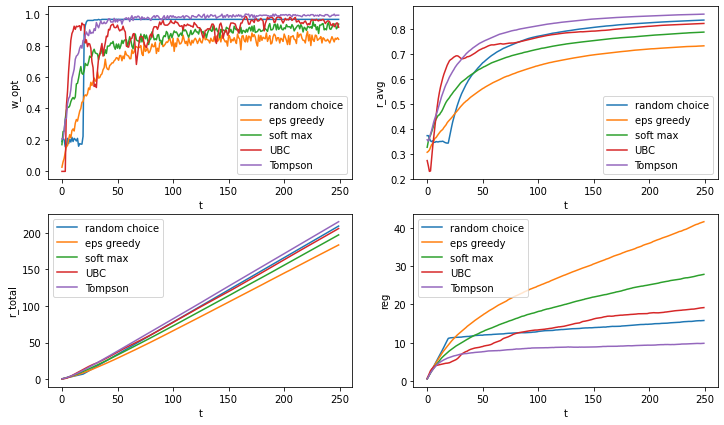
\includegraphics[width=10cm]{plots.png}

}

\end{document}
